%\documentclass{article}
%\usepackage[demo]{graphicx}
%\usepackage{subfig}
%\usepackage{tikz}
%\usepackage{multirow}
%\usepackage{siunitx}
%\begin{document}
%\begin{figure}
%\centering
%%%%%%%%%%%%%%%%%%%%%%%%%%%%%
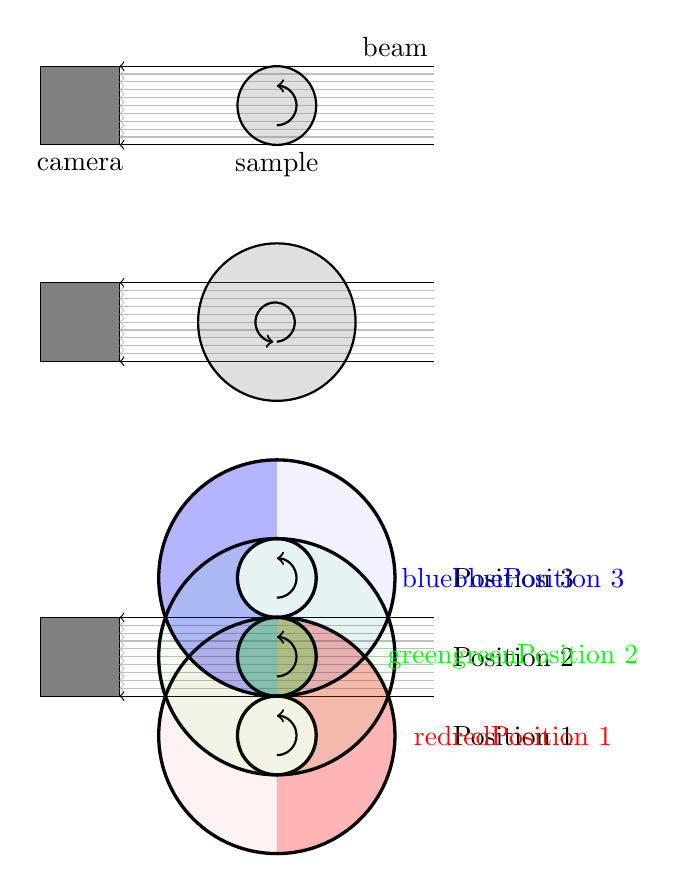
\begin{tikzpicture}
	%%%%%%%%%%%%%%%%%%%
	%      grid       %
	%%%%%%%%%%%%%%%%%%%
%		\def\stop{10}
%		\draw [color=gray] (0,0) grid (\stop,\stop);
%		\draw [shade] (0,0) circle (0.25) node {origin};
%		\draw [shade] (\stop,\stop) circle (0.25) node {\stop,\stop};
	%%%%%%%%%%%%%%%%%%%
	%       180       %
	%%%%%%%%%%%%%%%%%%%
		\def\startAtY{9}
		\def\BeamLength{4}
		\def\length{2}
		%camera
			\draw [fill=gray] (0,\startAtY) rectangle (1,\startAtY+1);
			\node at (0.5,\startAtY-.25) {camera};
		% beam
			% inner rays
			\foreach \x in {9,9.1,...,10}
				\draw[gray!50,<-] (1,\x) -- (\BeamLength+1,\x);
			% outer rays
			\foreach \x in {0,1}
				\draw[<-] (1,\startAtY+\x) -- (\BeamLength+1,\startAtY+\x);
			% label				
			\node at (\BeamLength+0.5,\startAtY+1+.25) {beam};
		%sample
			\fill [color=gray,nearly transparent] (0.5*\BeamLength+1,\startAtY+0.5) circle (0.5);
			\draw [thick] (0.5*\BeamLength+1,\startAtY+0.5) circle (0.5);
			\draw [thick,->] (0.5*\BeamLength+1,\startAtY+0.25)   arc (-90:90:0.25);
			\node at (0.5*\BeamLength+1,\startAtY-0.25) {sample};
	%%%%%%%%%%%%%%%%%%%
	%       360       %
	%%%%%%%%%%%%%%%%%%%
		\def\startAtY{6.25}
		%camera
			\draw [fill=gray] (0,\startAtY) rectangle (1,\startAtY+1);
%			\node at (0.5,\startAtY-.25) {camera};
		% beam
			% inner rays
			\foreach \x in {6.25,6.35,...,7.25}
				\draw[gray!50,<-] (1,\x) -- (\BeamLength+1,\x);
			% outer rays
			\foreach \x in {0,1}
				\draw[<-] (1,\startAtY+\x) -- (\BeamLength+1,\startAtY+\x);
			% label				
%			\node at (\BeamLength+0.5,\startAtY+1.25) {beam};
		%sample
			\fill [color=gray,nearly transparent] (0.5*\BeamLength+1,\startAtY+0.5) circle (1);
			\draw [thick] (0.5*\BeamLength+1,\startAtY+0.5) circle (1);
			\draw [thick,->] (0.5*\BeamLength+1,\startAtY+0.25) arc (-85:265:0.25);
%			\node at (0.5*\BeamLength+1,\startAtY-0.75) {sample};
	%%%%%%%%%%%%%%%%%%%
	% Wide Field Scan %
	%%%%%%%%%%%%%%%%%%%
		\def\startAtY{2}
		%camera
			\draw [fill=gray] (0,\startAtY) rectangle (1,\startAtY+1);
%			\node at (0.5,\startAtY-.25) {camera};
		% beam
			% inner rays
			\foreach \x in {2,2.1,...,3}
				\draw[gray!50,<-] (1,\x) -- (\BeamLength+1,\x);
			% outer rays
			\foreach \x in {0,1}
				\draw[<-] (1,\startAtY+\x) -- (\BeamLength+1,\startAtY+\x);
			% label				
%			\node at (\BeamLength+0.5,\startAtY+1.25) {beam};
		% shaded samples
		\fill [color=red,nearly transparent]   (0.5*\BeamLength+1,3)           arc (90:-90:1.5) -- ++(0,1) arc (-90:90:0.5);
		\fill [color=blue,nearly transparent]  (0.5*\BeamLength+1,3+2) arc (90:270:1.5) -- ++(0,1) arc (270:90:0.5);
		\fill [color=green,nearly transparent] (0.5*\BeamLength+1,3-0.5) circle (0.5);	
		\foreach \y/\position/\color in {\startAtY-0.5/1/red,\startAtY+0.5/2/green,\startAtY+1.5/3/blue}
			{
				\draw[very thick] (0.5*\BeamLength+1,\y) circle (1.5) circle (0.5);
				\draw[thick,->] (0.5*\BeamLength+1,\y-0.25) arc (-90:90:0.25);
				\fill [color=\color,ultra nearly transparent] (0.5*\BeamLength+1,\y) circle (1.5);
				\node at (\BeamLength+2+.005,\y-.005) {Position \position};
				\node [color=\color] at (\BeamLength+2,\y) {Position \position};
			}
\end{tikzpicture}
%%%%%%%%%%%%%%%%%%%%%%%%%%%%%	
%\caption{Caption}
%\end{figure}
%\end{document}